\documentclass[11pt,letterpaper]{article}

\usepackage[utf8]{inputenc}
\usepackage[T1]{fontenc}
\usepackage{lmodern}
\usepackage[margin=2.5cm]{geometry}
\usepackage{graphicx}
\usepackage{booktabs}
\usepackage{tabularx}
\usepackage{longtable}
\usepackage{array}
\usepackage{amssymb}
\usepackage{xcolor}
\usepackage{enumitem}
\usepackage{fancyhdr}
\usepackage{listings}
\usepackage{caption}
\usepackage{tikz}
\usetikzlibrary{positioning,arrows.meta,shapes.geometric}
\let\oldus\_
\renewcommand{\_}{\oldus\allowbreak}
\usepackage{xurl}
\usepackage[hidelinks]{hyperref}

\renewcommand{\contentsname}{Índice}
\renewcommand{\figurename}{Figura}
\renewcommand{\tablename}{Tabla}
\renewcommand{\lstlistingname}{Código}
\renewcommand{\refname}{Referencias}

\definecolor{usmblue}{RGB}{0,51,102}
\definecolor{okgreen}{RGB}{0,120,60}
\definecolor{partial}{RGB}{190,120,0}
\definecolor{nored}{RGB}{180,30,30}

\newcommand{\cumple}{Cumplido}
\newcommand{\parcial}{Parcial}
\newcommand{\nocumple}{No implementado}
\newcommand{\diferido}{Diferido}

\setlist[itemize]{label=\tiny$\blacksquare$, leftmargin=1.6em, itemsep=2pt, topsep=4pt}

\setlength{\parindent}{1.2em}
\setlength{\parskip}{2pt}
\setlength{\emergencystretch}{3em}
\renewcommand{\arraystretch}{1.15}

\pagestyle{fancy}
\fancyhf{}
\fancyhead[L]{\small Universidad Técnica Federico Santa María}
\fancyhead[R]{\small ICN-292 — Sistemas de Información para la Gestión}
\fancyfoot[C]{\thepage}
\renewcommand{\headrulewidth}{0.6pt}
\setlength{\headheight}{14pt}

\captionsetup{font=small}

\lstset{
  language=SQL, basicstyle=\ttfamily\small, keywordstyle=\bfseries\color{usmblue},
  numbers=left, numberstyle=\tiny\color{gray}, frame=single, rulecolor=\color{gray!50},
  breaklines=true, showstringspaces=false, columns=fullflexible, captionpos=b,
  literate={á}{{\'a}}1 {é}{{\'e}}1 {í}{{\'i}}1 {ó}{{\'o}}1 {ú}{{\'u}}1 {ñ}{{\~n}}1
}

\begin{document}

\begin{titlepage}
\thispagestyle{empty}
\centering
\vspace*{0.5cm}

\includegraphics[width=0.62\textwidth]{img/logo_usm.png}\par
\vspace{0.8cm}
{\small\textbf{DEPARTAMENTO DE INDUSTRIAS}\par
UNIVERSIDAD TÉCNICA FEDERICO SANTA MARÍA\par}
\vspace{1.6cm}
\rule{\textwidth}{0.6pt}\par\vspace{0.4cm}
{\huge Solución SIG para la Gestión\\[2pt] de Inventario\par}
\vspace{0.3cm}
{ICN-292 — Entrega 2\par}
\vspace{0.2cm}
{\itshape Caso: Comercial Electroliko SpA / La PicaOnline SpA (“Eliko”)\par}
\vspace{0.4cm}
\rule{\textwidth}{0.6pt}\par
\vspace{1.4cm}
\begin{tabular}{lll}
\toprule
\textbf{Nombre completo} & \textbf{Rol} & \textbf{Función en Proyecto} \\
\midrule
Rodrigo Barros     & 202360546-8 & Desarrollo del sistema y base de datos \\
Iovanni Fuentes    & 202360570-0 & Comunicación con la PYME y carga de base de datos \\
Benjamín Maturana  & 202304540-3 & Carga de base de datos y organización del inventario \\
Alonso López       & 202360535-2 & Carga de base de datos y organización del inventario \\
Maximiliano Uribe  & 202360533-6 & Carga de base de datos y organización del inventario \\
\bottomrule
\end{tabular}\par
\vspace{1.2cm}
Paralelo: 100\par
Enlace GitHub:\par
{\small\url{https://github.com/benjaminmaturanab-create/ICN292-GRUPO4-Barros-Fuentes-Lopez-Uribe-Maturana}}\par
\vspace{0.2cm}
Sistema en línea:\par
{\small\url{https://eliko-inventario-hcyyqk7oxjlhuwa94pkns2.streamlit.app}}\par
\vfill
Noviembre, 2026\par
\vspace{0.2cm}
Campus Vitacura\par
\end{titlepage}

\tableofcontents
\newpage

\section*{Resumen Ejecutivo}
\addcontentsline{toc}{section}{Resumen Ejecutivo}
\paragraph{Problema.} Eliko (Comercial Electroliko SpA / La PicaOnline SpA) vende por internet a través de cuatro canales (dos cuentas de Mercado Libre, Falabella y su página web), con cerca de 1.400 publicaciones activas y 800 ventas mensuales. No tenía un inventario centralizado: el stock se controlaba revisando físicamente los estantes y se actualizaba a mano en cada plataforma. Esto provocaba entre 3 y 4 cancelaciones de venta al mes por falta de stock, con pérdidas de \$100.000 a \$300.000 por cada una, además de la pausa automática de publicaciones en Mercado Libre.

\paragraph{Solución.} Se implementó un sistema de información para la gestión de inventario compuesto por cuatro partes:
\begin{itemize}
\item \textbf{Base de datos relacional en 3FN} (CATEGORIA, PRODUCTO, INVENTARIO y MOVIMIENTO\_STOCK) en SQLite, creada con \texttt{schema.sql} y cargada con \texttt{seed.sql}.
\item \textbf{Dashboard web} en Streamlit con 5 KPIs, stock por categoría, alertas de reposición, productos sin movimiento y búsqueda por SKU.
\item \textbf{Automatización con n8n:} un flujo revisa cada día los productos bajo su stock mínimo y envía un correo a Alejandro con la lista ordenada por urgencia.
\item \textbf{Cinco consultas SQL de negocio} sobre estado del inventario, alertas, quiebres por categoría, concentración del stock y productos en riesgo.
\end{itemize}
El proceso to-be se modeló en BPMN 2.0 con dos carriles (Encargado de Bodega y Sistema de Inventario) y dos decisiones: si el producto existe en el sistema y si su stock quedó bajo el mínimo.

\paragraph{Resultado.} El equipo levantó en terreno el inventario completo de la bodega: \textbf{767 productos} en \textbf{17 categorías}, con \textbf{8.964 unidades}. Por primera vez Eliko tiene una vista consolidada de su stock, y las consultas muestran información que antes no veía: \textbf{308 productos (40\%) están agotados}, con “Hogar y jardín” a la cabeza (132 de 194), mientras el 21\% de las unidades se concentra en solo 10 productos. También muestran el principal pendiente: solo 2 productos tienen stock mínimo definido, y hay 72 productos con 1 o 2 unidades que el sistema aún no puede alertar. Toda la solución es reproducible: basta clonar el repositorio y seguir el \texttt{README.md}.

\paragraph{Alcance.} La E2 resuelve la base del problema (saber cuánto stock hay y anticipar los quiebres), pero todavía no se conecta con los canales de venta. Por eso la venta simultánea de un mismo producto en dos plataformas aún no se elimina directamente; esa integración es el siguiente paso (§9).

\newpage

\section{Descripción de la Organización y Problemática de Gestión}
\subsection{Descripción de Eliko}
Eliko es una pequeña empresa comercial (PYME) dedicada a la importación y venta al por mayor y menor de productos de consumo masivo, organizados en 17 categorías que incluyen artículos del hogar, tecnología de consumo (cables, cargadores, accesorios para celular), artículos de oficina y otros productos de alta rotación.

La empresa gestiona actualmente un catálogo de \textbf{767 productos activos} distribuidos en \textbf{17 categorías}, con un stock total de \textbf{8.964 unidades} disponibles en bodega. Su operación depende de un encargado de bodega que registra manualmente entradas y salidas de mercancía.

\subsection{Diagnóstico: problemática de gestión}
El diagnóstico organizacional reveló las siguientes brechas críticas en la gestión de información:

\begin{description}[leftmargin=1.5em, style=nextline]
\item[Problema 1 — Ausencia de visibilidad del inventario en tiempo real.] La empresa no contaba con ningún sistema digital de seguimiento de stock. El control se realizaba mediante planillas físicas o archivos Excel sin estructura normalizada, lo que impedía conocer el estado real del inventario en un momento dado.
\item[Problema 2 — Gestión reactiva del reabastecimiento.] Sin alertas automáticas de stock mínimo, los pedidos de reposición se realizaban solo cuando el encargado detectaba físicamente la ausencia de un producto en bodega. Esto provocaba quiebres de stock que afectaban la operación comercial.
\item[Problema 3 — Falta de trazabilidad de movimientos.] No existía registro histórico de entradas y salidas, imposibilitando el análisis de demanda, la identificación de productos sin rotación y la planificación de compras futuras.
\item[Problema 4 — Inexistencia de KPIs operacionales.] La dirección no disponía de métricas consolidadas (total de unidades, distribución por categoría, alertas de reposición) para tomar decisiones de abastecimiento de forma informada.
\end{description}

\subsection{Propuesta de mejora}
Se propone el diseño e implementación de un \textbf{sistema de información de inventario} que digitalice el proceso completo de gestión de stock: registro de productos, control de entradas y salidas, generación automática de alertas de reposición y visualización de KPIs en un dashboard web accesible desde cualquier dispositivo.

\section{Trazabilidad Entrega 1 \texorpdfstring{$\rightarrow$}{->} Entrega 2}
Esta sección explica qué se mantuvo y qué cambió entre la propuesta de la Entrega 1 (E1) y la solución implementada en la Entrega 2 (E2), y por qué. Se recorre cada producto de la E1 en el mismo orden en que fue presentado: problema, requerimientos, BPMN, modelo de datos, arquitectura y plan de trabajo.

\subsection{Visión general: qué se mantuvo y qué cambió}

\begin{center}
\small
\begin{tabularx}{\textwidth}{>{\raggedright\arraybackslash}p{2.6cm} >{\raggedright\arraybackslash}X >{\raggedright\arraybackslash}X}
\toprule
\textbf{Elemento} & \textbf{Entrega 1 (propuesta)} & \textbf{Entrega 2 (implementado)} \\
\midrule
PYME y problema & Eliko; falta de inventario centralizado entre 4 canales; 3–4 cancelaciones al mes por quiebre de stock (pérdida de \$100.000 a \$300.000 c/u). & Se mantiene la misma PYME y el mismo problema de fondo: no saber cuánto stock hay y reaccionar tarde a los quiebres. \\
Alcance & Inventario consolidado \emph{multicanal}: ingresos, ventas por canal, publicaciones, cancelaciones y alertas. & Inventario consolidado de la \emph{bodega}: productos, categorías, entradas/salidas y alertas. Los canales quedan para una etapa siguiente. \\
BPMN to-be & Proceso de venta, inventario y despacho con 5+ actores y un carril “Sistema de gestión SIG”. & Proceso de registro de movimientos de bodega con 2 carriles (Encargado de bodega y Sistema) y 2 gateways XOR. \\
Modelo de datos & 10 entidades preliminares (Producto, Variante, Canal, Publicación, Proveedor, IngresoStock, Venta, DetalleVenta, Cancelación, AlertaStock). & 4 tablas en 3FN (CATEGORIA, PRODUCTO, INVENTARIO, MOVIMIENTO\_STOCK). \\
Stack & React + Node/Express + PostgreSQL 16 + Docker Compose. & Python + Streamlit + SQLite 3, desplegado en Streamlit Community Cloud. \\
Datos & Plan: datos reales o simulados (hito H6). & Datos reales: inventario físico levantado en terreno (767 productos, octubre 2026). \\
\bottomrule
\end{tabularx}
\end{center}

\paragraph{Por qué se redujo el alcance.} En la E1 ya se habían identificado dos condiciones que hacían inviable la versión multicanal completa en un semestre: la integración vía API con cada plataforma estaba clasificada como \emph{Won't} (RF10), y el riesgo “datos históricos incompletos o poco confiables” tenía como mitigación \emph{partir con un conteo físico único de stock inicial}. La E2 sigue exactamente esa mitigación: antes de conectar canales, el negocio necesita una base de inventario confiable, porque sin ella cualquier descuento automático por venta se aplicaría sobre un stock incorrecto. Por eso se priorizó construir y validar esa base (767 productos inventariados en terreno), dejando la capa multicanal como evolución.

\subsection{Requerimientos: estado de implementación}
La Tabla~\ref{tab:rf} recorre los requisitos funcionales priorizados con MoSCoW en la E1 e indica cómo quedó cada uno en la E2. Se consideran todos los \emph{Must} y se explica la brecha de los que no se completaron.

\begin{small}
\begin{longtable}{>{\raggedright\arraybackslash}p{1.0cm} >{\raggedright\arraybackslash}p{3.7cm} >{\raggedright\arraybackslash}p{1.1cm} >{\raggedright\arraybackslash}p{2.0cm} >{\raggedright\arraybackslash}p{5.2cm}}
\caption{Trazabilidad de requisitos funcionales E1 $\rightarrow$ E2.}\label{tab:rf}\\
\toprule
\textbf{ID} & \textbf{Requisito (E1)} & \textbf{Prior.} & \textbf{Estado E2} & \textbf{Cómo se cumple / por qué no} \\
\midrule
\endfirsthead
\toprule
\textbf{ID} & \textbf{Requisito (E1)} & \textbf{Prior.} & \textbf{Estado E2} & \textbf{Cómo se cumple / por qué no} \\
\midrule
\endhead
\bottomrule
\endfoot
RF01 & Registrar ingreso de mercadería (producto, variante, cantidad, fecha, proveedor). & Must & \parcial & El modelo lo soporta: \texttt{movimiento\_stock} admite ENTRADA con cantidad, fecha y motivo, y cada variante es un SKU propio. Falta un formulario en el dashboard; hoy los movimientos se registran por SQL. \\
RF02 & Descontar stock automáticamente al registrar una venta en cualquier canal. & Must & \parcial & El modelo registra SALIDAS y guarda el stock en \texttt{inventario}, pero el descuento automático no está implementado (no hay formulario ni trigger). Tampoco se guarda el canal. \\
RF03 & Mostrar stock consolidado por producto y variante, visible para todo el equipo. & Must & \cumple & Dashboard web con KPIs (767 productos, 8.964 unidades) y stock por categoría, accesible desde cualquier dispositivo. \\
RF04 & Alerta cuando el stock cae bajo un umbral configurable. & Must & \cumple & Umbral \texttt{stock\_minimo} por producto; alerta en el dashboard y correo diario vía n8n. Hoy solo 2 productos tienen umbral definido (§6.5). \\
RF05 & Registro manual de ventas en canales sin integración. & Should & \nocumple & El dashboard no tiene formulario de registro (§9.2). \\
RF06 & Asociar un producto físico con sus publicaciones en cada canal. & Should & \diferido & Requiere las entidades Canal y Publicación; queda para la siguiente etapa junto con la capa multicanal. \\
RF07 & Reportes de rotación y de cancelaciones por falta de stock. & Should & \parcial & Productos sin movimiento en el dashboard y quiebres por categoría (§6.3). Cancelaciones: no se modelaron. \\
RF08 & Registrar el motivo de cada cancelación. & Could & \diferido & Depende de la entidad Venta/Cancelación (no implementada). \\
RF09 & Priorizar reposición según historial de ventas y stock crítico. & Could & \parcial & Las alertas se ordenan por unidades a reponer y la §6.5 identifica los productos críticos; falta ponderar por historial de ventas. \\
RF10 & Integración automática vía API con cada plataforma. & Won't & \diferido & Fuera de alcance desde la E1; se mantiene como evolución futura. \\
\end{longtable}
\end{small}

\begin{small}
\begin{longtable}{>{\raggedright\arraybackslash}p{1.2cm} >{\raggedright\arraybackslash}p{4.0cm} >{\raggedright\arraybackslash}p{2.0cm} >{\raggedright\arraybackslash}p{6.6cm}}
\caption{Trazabilidad de requisitos no funcionales E1 $\rightarrow$ E2.}\\
\toprule
\textbf{ID} & \textbf{Requisito no funcional (E1)} & \textbf{Estado E2} & \textbf{Evidencia} \\
\midrule
\endfirsthead
\toprule
\textbf{ID} & \textbf{Requisito no funcional (E1)} & \textbf{Estado E2} & \textbf{Evidencia} \\
\midrule
\endhead
\bottomrule
\endfoot
RNF01 & Disponibilidad en horario de trabajo. & \cumple & Sistema desplegado en Streamlit Community Cloud, disponible 24/7. \\
RNF02 & Registrar un movimiento en pocos pasos, sin capacitación técnica. & \parcial & El dashboard es simple de consultar, pero registrar movimientos aún requiere SQL (falta el formulario). \\
RNF03 & Consulta de stock prácticamente inmediata. & \cumple & SQLite responde en milisegundos con el volumen actual (767 productos). \\
RNF04 & Protección de datos según Ley 21.719. & \parcial & La E2 no almacena datos de clientes (reduce el riesgo); falta autenticación. \\
RNF05 & Soportar el volumen actual y su crecimiento. & \cumple & El volumen actual es bajo para SQLite; migrar a PostgreSQL queda como opción si crece. \\
RNF06 & Consulta desde dispositivo móvil. & \cumple & Aplicación web accesible desde el navegador del celular. \\
\end{longtable}
\end{small}

\subsection{Proceso BPMN: cambios respecto del to-be de la E1}
El BPMN to-be de la E1 modelaba el proceso completo de \emph{venta, control de inventario y despacho}, con carriles para Alejandro, su pareja, el operador de despacho, los canales de venta y un carril nuevo “Sistema de gestión SIG”. El BPMN final de la E2 (Figura~\ref{fig:bpmn}) se concentra en la parte de ese proceso que el sistema implementado realmente ejecuta:

\begin{itemize}
\item \textbf{Se mantiene:} el carril del sistema que descuenta stock, evalúa el umbral mínimo y genera la alerta. Es el núcleo de las mejoras “qué se automatiza” y “qué se controla” de la E1 (§3.3 de la E1).
\item \textbf{Se simplifica:} los carriles humanos se agrupan en un solo actor, el \emph{Encargado de Bodega}, que es quien registra entradas y salidas.
\item \textbf{Se agrega:} el gateway “¿Existe en sistema?”, que obliga a registrar un producto nuevo antes de moverlo. No existía en la E1 y asegura la integridad referencial con \texttt{movimiento\_stock}.
\item \textbf{Se automatiza:} la tarea “Generar alerta” se implementa con un flujo n8n que revisa el stock cada día y notifica a Alejandro por correo (§3.4). En la E1 esta tarea estaba planificada con \texttt{node-cron} dentro del backend.
\item \textbf{Se posterga:} la recepción de ventas desde los canales, la preparación y el despacho, y la generación del reporte semanal. Siguen fuera del sistema mientras no exista la capa multicanal.
\end{itemize}

\subsection{Modelo de datos: de 10 entidades preliminares a 4 tablas en 3FN}
La Tabla~\ref{tab:er} muestra qué pasó con cada entidad del modelo preliminar de la E1.

\begin{small}
\begin{longtable}{>{\raggedright\arraybackslash}p{2.3cm} >{\raggedright\arraybackslash}p{3.9cm} >{\raggedright\arraybackslash}p{8.9cm}}
\caption{Evolución de las entidades del modelo de datos.}\label{tab:er}\\
\toprule
\textbf{Entidad E1} & \textbf{En la E2} & \textbf{Justificación} \\
\midrule
\endfirsthead
\toprule
\textbf{Entidad E1} & \textbf{En la E2} & \textbf{Justificación} \\
\midrule
\endhead
\bottomrule
\endfoot
Producto & PRODUCTO & Se mantiene, con el SKU de bodega como clave primaria (ej.: HOG001). \\
Variante & Integrada en PRODUCTO & Cada variante ya tiene su propio SKU en el inventario físico (ej.: HOG025B, CTR007G), así que no necesita una tabla aparte. \\
\emph{stock} (en Variante) & INVENTARIO (tabla nueva) & El stock actual, el mínimo y la fecha del último conteo se separan del catálogo, en relación 1:1 con PRODUCTO (§4.3). \\
\emph{categoría} (atributo) & CATEGORIA (entidad) & Mejora de normalización: en la E1 era un texto dentro de Producto. Como entidad propia se evita la anomalía de actualización (§4.3). \\
IngresoStock & MOVIMIENTO\_STOCK & Entradas, salidas y ajustes se unifican en una tabla con \texttt{tipo\_movimiento}, validado con CHECK. \\
Venta / DetalleVenta & MOVIMIENTO\_STOCK (SALIDA) & La salida de bodega cumple el rol de descontar stock; el encabezado de venta por canal queda diferido. \\
AlertaStock & Consulta SQL & La alerta no se almacena: se calcula con \texttt{stock\_actual < stock\_minimo}. Así nunca queda desactualizada. \\
Canal, Publicación & Diferidas & Necesarias para RF06 y la capa multicanal. \\
Proveedor & Diferida & No forma parte del inventario levantado en terreno. \\
Cancelación & Diferida & Depende de Venta; necesaria para RF07–RF08. \\
\end{longtable}
\end{small}

\subsection{Arquitectura y stack tecnológico}
\begin{center}
\small
\begin{tabularx}{\textwidth}{>{\raggedright\arraybackslash}p{2.6cm} >{\raggedright\arraybackslash}p{3.6cm} >{\raggedright\arraybackslash}p{3.2cm} >{\raggedright\arraybackslash}X}
\toprule
\textbf{Capa} & \textbf{E1 (tentativo)} & \textbf{E2 (implementado)} & \textbf{Motivo del cambio} \\
\midrule
Interfaz & React + Vite + Tailwind & Streamlit & Un solo lenguaje (Python) para interfaz, lógica y visualización; menos código que mantener. \\
Lógica / backend & Node.js + Express + node-cron & Python (dentro de \texttt{app.py}) & La lógica de negocio (descontar stock, evaluar umbral) cabe en la misma aplicación; no se justificaba una API separada. \\
Base de datos & PostgreSQL 16 + Prisma & SQLite 3 & Archivo \texttt{.sql} reproducible sin instalar un servidor; suficiente para el volumen actual. \\
Despliegue & Docker Compose en localhost & Streamlit Community Cloud & Despliegue gratuito y accesible desde cualquier dispositivo; la base se regenera sola desde el script SQL al iniciar. \\
Automatización & Tarea programada con \texttt{node-cron} & Flujo en n8n Cloud (§3.4) & Herramienta del curso; el flujo es visible, editable sin programar y queda trazado a la tarea del BPMN. \\
\bottomrule
\end{tabularx}
\end{center}

Lo que se mantiene de la E1 es el objetivo de \textbf{reproducibilidad}: en la E1 se buscaba con \texttt{docker compose up}; en la E2 se logra versionando el script SQL (texto plano) y regenerando la base automáticamente al iniciar la aplicación (§5).

\subsection{Plan de la Entrega 2: cumplimiento de hitos}
\begin{center}
\small
\begin{tabularx}{\textwidth}{>{\raggedright\arraybackslash}p{0.8cm} >{\raggedright\arraybackslash}p{5.0cm} >{\raggedright\arraybackslash}p{2.4cm} >{\raggedright\arraybackslash}X}
\toprule
\textbf{Hito} & \textbf{Descripción (E1)} & \textbf{Estado} & \textbf{Comentario} \\
\midrule
H1 & Entorno Docker Compose reproducible. & Reemplazado & Se reemplazó por Streamlit Cloud + autoinicialización de la base. \\
H2 & Crear la base de datos según el ER. & \cumple & Base SQLite en 3FN con 4 tablas, \texttt{schema.sql} y \texttt{seed.sql}. \\
H3 & RF01–RF04 (ingreso, descuento, consulta, alertas). & \parcial & Consulta y alertas implementadas; el registro y descuento de movimientos está modelado pero sin formulario. \\
H4 & RF05–RF07 (venta manual, multicanal, reportes). & \parcial & Reporte de rotación implementado; multicanal diferido. \\
H5 & Panel web (dashboard, formularios, alertas). & \cumple & Dashboard con 5 KPIs, gráficos y tablas. \\
H6 & Cargar datos reales o simulados y probar con Alejandro. & \parcial & Datos reales cargados (inventario de octubre 2026). \\
H7 & RF08–RF09 si el tiempo lo permite. & \parcial & Priorización por déficit; motivo de cancelación diferido. \\
H8 & Documentación, README y presentación. & \cumple & Este informe, README y presentación de la defensa. \\
\bottomrule
\end{tabularx}
\end{center}

\subsection{Riesgos identificados en la E1: qué ocurrió}
\begin{itemize}
\item \textbf{Datos históricos incompletos.} Se materializó: no existía un registro confiable de stock. Se aplicó la mitigación planificada: un conteo físico único en terreno, que dio origen al archivo \texttt{Inventario\_Bodega\_Eliko\_14\_10\_2026.csv}.
\item \textbf{Datos personales de clientes (Ley 21.719).} Se redujo: al no implementarse Venta, el sistema no almacena nombres, direcciones ni teléfonos de clientes. Las medidas de la E1 (control de acceso por rol, plazo de conservación, cifrado) siguen vigentes para cuando se agregue la capa de ventas.
\item \textbf{Resistencia al cambio.} Se abordó con una interfaz web simple (RNF02).
\item \textbf{Dependencia de un solo integrante en backend/BD.} Se mitiga documentando el modelo (§4), las consultas (§6) y el repositorio (§7) para que cualquier integrante pueda continuar el trabajo.
\end{itemize}

\subsection{Repositorio}
El proyecto tiene un \textbf{repositorio único} para ambas entregas, el mismo de la E1 (\url{https://github.com/benjaminmaturanab-create/ICN292-GRUPO4-Barros-Fuentes-Lopez-Uribe-Maturana}). La E2 agrega el sistema, la base de datos, las consultas, la automatización y la documentación \texttt{.md}, sin borrar los entregables de la E1; el detalle de los cambios está en \texttt{CHANGELOG.md}. La versión en línea del dashboard se publica en Streamlit Community Cloud a partir de una copia del mismo código.

\section{Modelado del Proceso — Diagrama BPMN 2.0}
\subsection{Descripción del proceso modelado}
El proceso modelado corresponde a la \textbf{Gestión de Inventario en Bodega}: desde la recepción de un producto hasta la actualización del stock y la generación de alertas de reposición cuando corresponda.

\subsection{Diagrama BPMN}
\begin{figure}[h]
\centering
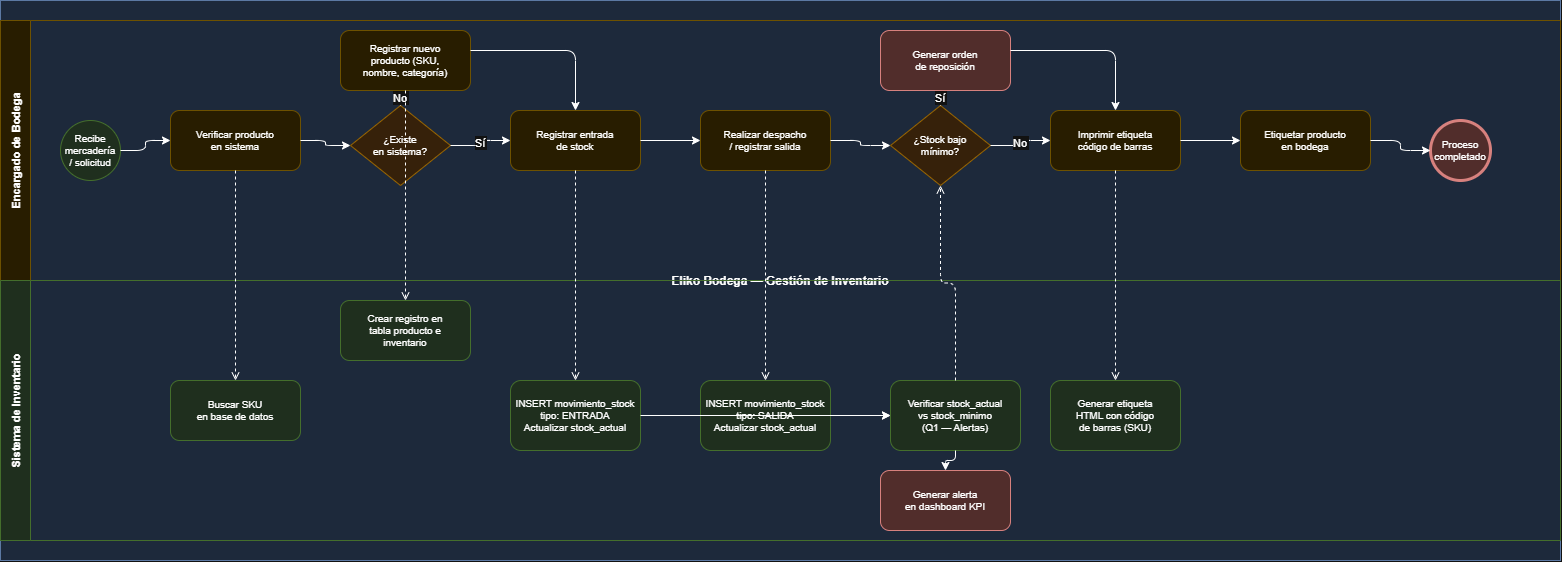
\includegraphics[width=\textwidth]{img/bpmn.png}
\caption{Diagrama BPMN 2.0 — Gestión de Inventario Eliko.}\label{fig:bpmn}
\end{figure}

El diagrama BPMN 2.0 representa el proceso completo con los siguientes elementos.

\textbf{Carriles (lanes):}
\begin{itemize}
\item \textbf{Encargado de Bodega:} actor humano responsable de registrar los movimientos físicos de mercancía.
\item \textbf{Sistema de Inventario:} sistema computacional que valida, persiste y controla la lógica de negocio.
\end{itemize}

\textbf{Flujo del proceso:}
\begin{enumerate}[leftmargin=1.6em]
\item \textbf{Inicio:} el encargado recibe mercancía o registra una salida de bodega.
\item \textbf{Verificación de existencia} (\emph{Gateway XOR — “¿Existe en sistema?”}):
  \begin{itemize}
  \item \textbf{Sí:} el sistema procede a registrar el movimiento.
  \item \textbf{No:} se debe registrar el nuevo producto antes de continuar (\texttt{INSERT INTO producto}).
  \end{itemize}
\item \textbf{Registro del movimiento:} el sistema ejecuta \texttt{INSERT INTO movimiento\_stock} con tipo, cantidad y fecha.
\item \textbf{Actualización del stock:} el sistema ejecuta \texttt{UPDATE inventario SET stock\_actual}.
\item \textbf{Verificación de stock mínimo} (\emph{Gateway XOR — “¿Stock bajo mínimo?”}):
  \begin{itemize}
  \item \textbf{Sí:} se genera una alerta visible en el dashboard.
  \item \textbf{No:} el proceso concluye sin acción adicional.
  \end{itemize}
\item \textbf{Fin:} el inventario queda actualizado y el dashboard refleja el estado actual.
\end{enumerate}

\subsection{Justificación del diseño}
La separación en dos carriles refleja la distinción fundamental entre el actor humano (que toma la decisión operativa) y el sistema (que ejecuta la lógica de negocio y persiste los datos). Los dos gateways XOR capturan las dos decisiones críticas del proceso: (1) si el producto es nuevo para el sistema, y (2) si el stock resultante requiere acción de reposición.

\subsection{Automatización del proceso con n8n}
La tarea \textbf{“Generar alerta”} del carril \emph{Sistema de Inventario}, que sigue a la salida “Sí” del gateway \textbf{“¿Stock bajo mínimo?”}, se automatizó con un flujo de n8n. Sin esta automatización, la alerta solo aparece si alguien abre el dashboard; con ella, Alejandro recibe un correo cada mañana con los productos que debe reponer, sin tener que buscarlos.

\begin{figure}[h]
\centering
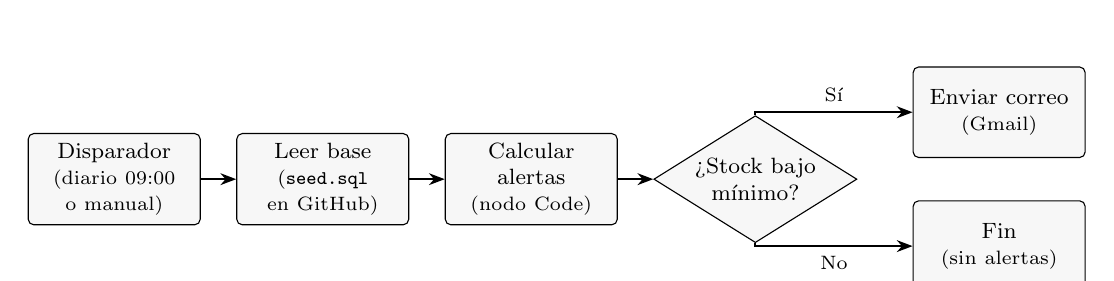
\begin{tikzpicture}[
  nodo/.style={draw, rounded corners=2pt, align=center, font=\footnotesize, minimum height=1.15cm, text width=1.95cm, fill=gray!6},
  dec/.style={draw, diamond, aspect=1.6, align=center, font=\footnotesize, inner sep=1pt, text width=1.55cm, fill=gray!6},
  flecha/.style={-{Stealth[length=2mm]}, thick},
  node distance=0.45cm]
\node[nodo] (t) {Disparador\\\scriptsize(diario 09:00 o manual)};
\node[nodo, right=of t] (q) {Leer base\\\scriptsize(\texttt{seed.sql} en GitHub)};
\node[nodo, right=of q] (c) {Calcular alertas\\\scriptsize(nodo Code)};
\node[dec, right=of c] (d) {¿Stock bajo mínimo?};
\node[nodo, right=0.7cm of d, yshift=0.85cm] (g) {Enviar correo\\\scriptsize(Gmail)};
\node[nodo, right=0.7cm of d, yshift=-0.85cm] (f) {Fin\\\scriptsize(sin alertas)};
\draw[flecha] (t) -- (q);
\draw[flecha] (q) -- (c);
\draw[flecha] (c) -- (d);
\draw[flecha] (d.north) |- node[pos=0.75, above, font=\scriptsize] {Sí} (g.west);
\draw[flecha] (d.south) |- node[pos=0.75, below, font=\scriptsize] {No} (f.west);
\end{tikzpicture}
\caption{Flujo n8n “Eliko — Alerta de stock bajo mínimo”.}\label{fig:n8n}
\end{figure}

\begin{small}
\begin{longtable}{>{\raggedright\arraybackslash}p{3.3cm} >{\raggedright\arraybackslash}p{2.5cm} >{\raggedright\arraybackslash}p{9.2cm}}
\caption{Nodos del flujo n8n y su traza al BPMN.}\label{tab:n8n}\\
\toprule
\textbf{Nodo n8n} & \textbf{Tipo} & \textbf{Qué hace / elemento BPMN} \\
\midrule
\endfirsthead
\toprule
\textbf{Nodo n8n} & \textbf{Tipo} & \textbf{Qué hace / elemento BPMN} \\
\midrule
\endhead
\bottomrule
\endfoot
Todos los días 09:00 / Ejecución manual & Schedule Trigger / Manual Trigger & Inicia la revisión cada mañana, antes de la preparación de pedidos. El disparador manual permite demostrarlo en la defensa. \\
Leer base de datos (seed.sql en GitHub) & HTTP Request & Descarga \texttt{seed.sql} desde el repositorio público del proyecto. \\
Calcular alertas y armar mensaje & Code (JavaScript) & Lee las tablas CATEGORIA, PRODUCTO e INVENTARIO del seed y aplica la misma regla que la Consulta 2 (§6.2): \texttt{stock\_minimo} definido y \texttt{stock\_actual < stock\_minimo}, ordenado por déficit. Arma el correo con una tabla (código, producto, categoría, stock, mínimo y déficit). \\
¿Stock bajo mínimo? & IF & Corresponde al gateway XOR del mismo nombre en el BPMN: continúa solo si hay al menos un producto bajo su mínimo. \\
Enviar alerta por correo (Gmail) & Gmail & Corresponde a la tarea \textbf{“Generar alerta”}: envía el correo a Alejandro con la lista de reposición. \\
Sin alertas: fin & No Operation & Corresponde al evento de fin cuando el stock está sobre el mínimo: no se envía nada. \\
\end{longtable}
\end{small}

\paragraph{Por qué leer el seed desde GitHub.} El flujo corre en n8n Cloud, que no puede ejecutar comandos ni leer archivos de un computador. Por eso descarga \texttt{seed.sql} del repositorio y evalúa la regla de alerta en un nodo de código. Se verificó que el nodo entrega los mismos resultados que la base SQLite: 767 productos, 1 alerta (HOG001, déficit 50), 308 agotados y 72 productos críticos sin umbral, igual que las Consultas 1, 2 y 5 (§6). Como corre en la nube, la alerta se envía todos los días aunque ningún computador del equipo esté encendido. El flujo se ejecutó en la instancia de n8n Cloud del equipo el 20/11/2026 y el correo de alerta llegó correctamente (Figura~\ref{fig:n8nrun}).

\paragraph{Evidencia en el repositorio.} El flujo exportado está en \path{n8n/flujo_alerta_stock_cloud.json} (se importa en n8n con \emph{Import from File}) y su documentación paso a paso en \path{docs/05-automatizacion-n8n.md}. El repositorio incluye además una versión para n8n local que consulta \texttt{eliko.db} con \texttt{scripts/alertas\_stock.py}.

\begin{figure}[h]
\centering
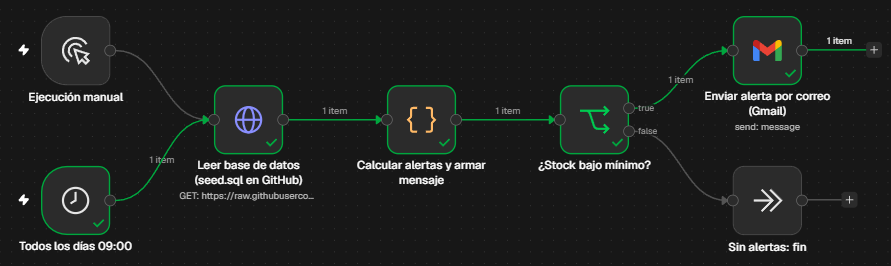
\includegraphics[width=\textwidth]{img/n8n_ejecucion.png}\\[0.4cm]
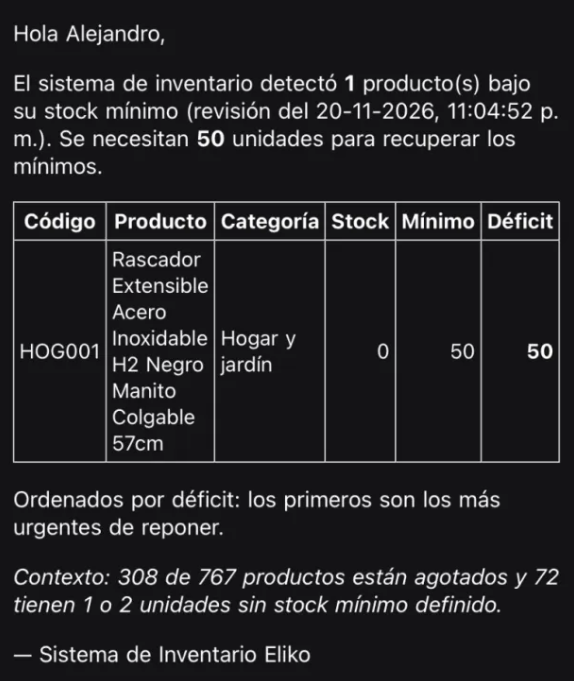
\includegraphics[width=0.5\textwidth]{img/n8n_correo.png}
\caption{Ejecución del flujo en n8n Cloud (arriba) y correo de alerta recibido (abajo), 20/11/2026.}\label{fig:n8nrun}
\end{figure}

\section{Modelo Entidad-Relación Normalizado (3FN)}
\subsection{Diagrama entidad-relación}
\begin{figure}[h]
\centering
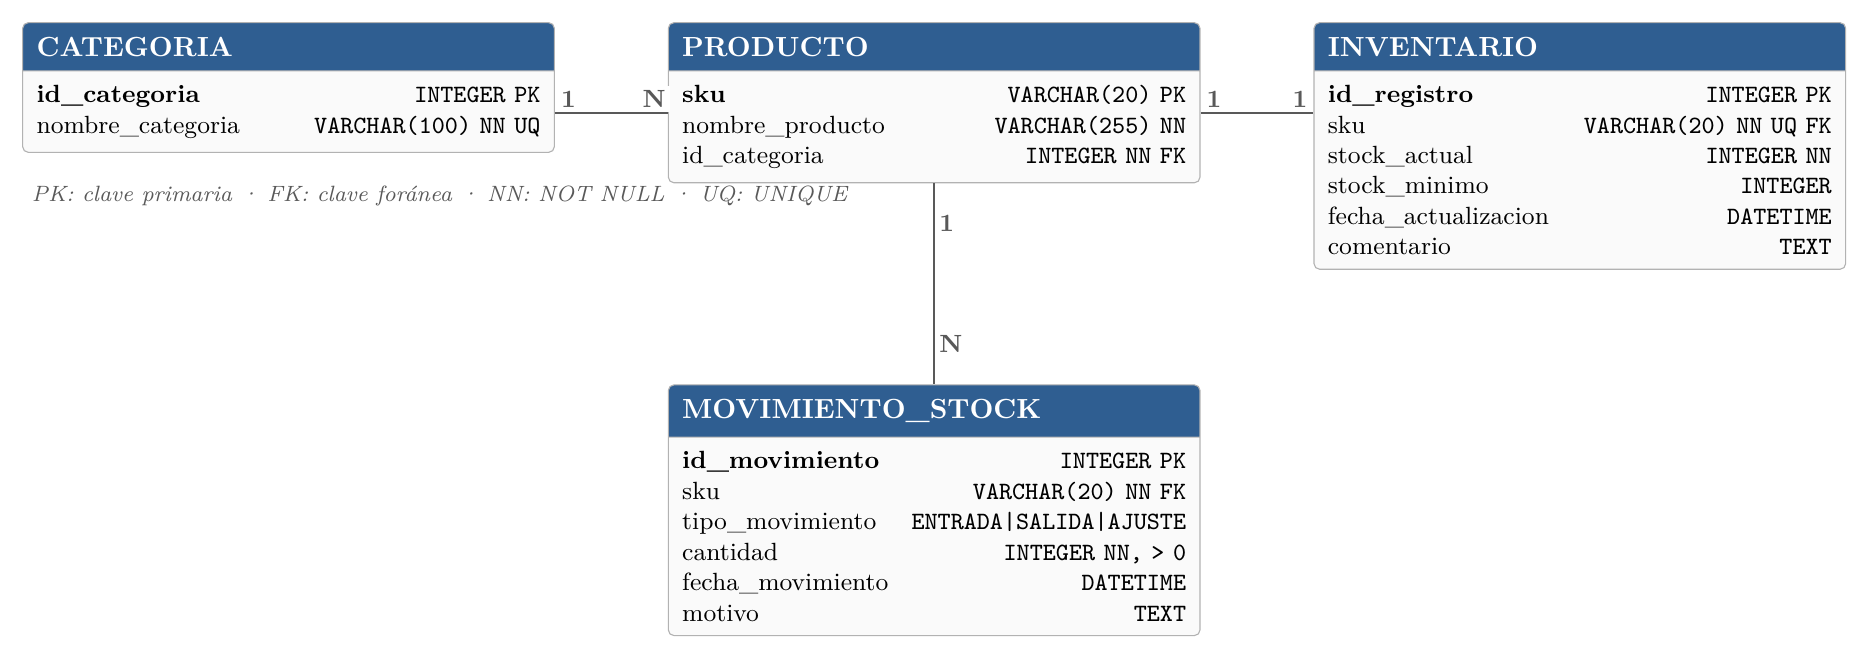
\includegraphics[width=\textwidth]{img/er.png}
\caption{Modelo entidad-relación implementado en \texttt{schema.sql}.}\label{fig:er}
\end{figure}

El modelo tiene cuatro tablas:
\begin{itemize}
\item \textbf{CATEGORIA (1) $\rightarrow$ PRODUCTO (N):} cada producto pertenece a una categoría; una categoría agrupa muchos productos.
\item \textbf{PRODUCTO (1) $\rightarrow$ INVENTARIO (1):} cada producto tiene exactamente un registro de stock (\texttt{sku} es \texttt{UNIQUE} en INVENTARIO).
\item \textbf{PRODUCTO (1) $\rightarrow$ MOVIMIENTO\_STOCK (N):} cada movimiento referencia un producto; un producto acumula su historial de movimientos.
\end{itemize}

\subsection{Diccionario de datos}
\begin{center}
\small
\begin{minipage}{\textwidth}\centering
\captionof{table}{Tabla CATEGORIA.}
\begin{tabularx}{\textwidth}{>{\ttfamily}l l X}
\toprule
\textrm{\textbf{Atributo}} & \textbf{Tipo / regla} & \textbf{Descripción} \\
\midrule
id\_categoria & INTEGER, PK, autoincremental & Identificador de la categoría \\
nombre\_categoria & VARCHAR(100), NOT NULL, UNIQUE & Nombre (ej.: Hogar y jardín). UNIQUE evita categorías duplicadas \\
\bottomrule
\end{tabularx}
\end{minipage}

\vspace{0.5cm}
\begin{minipage}{\textwidth}\centering
\captionof{table}{Tabla PRODUCTO.}
\begin{tabularx}{\textwidth}{>{\ttfamily}l l X}
\toprule
\textrm{\textbf{Atributo}} & \textbf{Tipo / regla} & \textbf{Descripción} \\
\midrule
sku & VARCHAR(20), PK & Código del producto usado en bodega (ej.: HOG001). Cada variante tiene su propio SKU (ej.: CTR007G) \\
nombre\_producto & VARCHAR(255), NOT NULL & Nombre descriptivo \\
id\_categoria & INTEGER, NOT NULL, FK & Referencia a CATEGORIA \\
\bottomrule
\end{tabularx}
\end{minipage}

\vspace{0.5cm}
\begin{minipage}{\textwidth}\centering
\captionof{table}{Tabla INVENTARIO.}
\begin{tabularx}{\textwidth}{>{\ttfamily}l l X}
\toprule
\textrm{\textbf{Atributo}} & \textbf{Tipo / regla} & \textbf{Descripción} \\
\midrule
id\_registro & INTEGER, PK, autoincremental & Identificador del registro de stock \\
sku & VARCHAR(20), NOT NULL, UNIQUE, FK & Producto al que corresponde (uno a uno) \\
stock\_actual & INTEGER, NOT NULL, DEFAULT 0 & Unidades disponibles en bodega \\
stock\_minimo & INTEGER, puede ser NULL & Umbral de alerta. NULL significa “sin umbral definido” \\
fecha\_actualizacion & DATETIME & Último conteo o actualización \\
comentario & TEXT & Observaciones del conteo \\
\bottomrule
\end{tabularx}
\end{minipage}

\vspace{0.5cm}
\begin{minipage}{\textwidth}\centering
\captionof{table}{Tabla MOVIMIENTO\_STOCK.}
\begin{tabularx}{\textwidth}{>{\ttfamily}l l X}
\toprule
\textrm{\textbf{Atributo}} & \textbf{Tipo / regla} & \textbf{Descripción} \\
\midrule
id\_movimiento & INTEGER, PK, autoincremental & Identificador del movimiento \\
sku & VARCHAR(20), NOT NULL, FK & Producto movido \\
tipo\_movimiento & CHECK IN ('ENTRADA','SALIDA','AJUSTE') & Tipo de movimiento; el CHECK impide valores inválidos \\
cantidad & INTEGER, NOT NULL, CHECK > 0 & Unidades movidas; el CHECK impide cantidades negativas o cero \\
fecha\_movimiento & DATETIME, DEFAULT CURRENT\_TIMESTAMP & Fecha y hora \\
motivo & TEXT & Motivo (venta, recepción, corrección de conteo, etc.) \\
\bottomrule
\end{tabularx}
\end{minipage}
\end{center}

Además, \texttt{schema.sql} crea tres índices: por categoría del producto, por SKU del movimiento y por fecha del movimiento, que aceleran las consultas por categoría y el historial de cada producto.

\subsection{Verificación de normalización (3FN)}
\begin{center}
\small
\captionof{table}{Verificación de formas normales.}
\begin{tabularx}{\textwidth}{l X}
\toprule
\textbf{Forma normal} & \textbf{Verificación} \\
\midrule
1FN \checkmark & Todos los atributos son atómicos. No hay grupos repetitivos: los movimientos de un producto son filas de MOVIMIENTO\_STOCK, no columnas de PRODUCTO. \\
2FN \checkmark & Todas las claves primarias son simples (un solo atributo), por lo que no puede haber dependencias parciales. \\
3FN \checkmark & No hay dependencias transitivas: el nombre de la categoría vive solo en CATEGORIA (PRODUCTO guarda la FK), y los datos de stock dependen solo del registro de INVENTARIO de ese SKU. \\
\bottomrule
\end{tabularx}
\end{center}

\textbf{Anomalías evitadas.}
\begin{itemize}
\item \emph{Actualización:} si la categoría fuera un texto dentro de PRODUCTO, renombrarla obligaría a modificar hasta 194 filas (las de “Hogar y jardín”). Con CATEGORIA se cambia un solo registro.
\item \emph{Inserción:} gracias a la FK, no se puede registrar un movimiento de un SKU que no existe; por eso el BPMN exige registrar primero el producto (gateway “¿Existe en sistema?”).
\item \emph{Datos inválidos:} los CHECK de MOVIMIENTO\_STOCK rechazan tipos de movimiento desconocidos y cantidades menores o iguales a cero.
\end{itemize}

\textbf{Por qué INVENTARIO es una tabla aparte.} PRODUCTO guarda datos de catálogo que casi no cambian (nombre, categoría), mientras INVENTARIO guarda el estado de bodega, que cambia con cada conteo o movimiento. Separarlas permite actualizar el stock sin tocar el catálogo y registrar la fecha y el comentario de cada conteo.

\textbf{Dato derivado controlado.} \texttt{stock\_actual} podría calcularse sumando los movimientos, pero se almacena porque el punto de partida es un conteo físico, no un historial. Desde ese conteo, cada movimiento debe actualizarlo; si hubiera diferencias, se corrigen con un movimiento de tipo AJUSTE, que deja trazabilidad.

\section{Sistema de Información Desarrollado}
El sistema es un \textbf{dashboard web} construido con Python y Streamlit sobre la base SQLite, publicado en Streamlit Community Cloud (\url{https://eliko-inventario-hcyyqk7oxjlhuwa94pkns2.streamlit.app}). Muestra 5 KPIs (productos, categorías, unidades, alertas activas y movimientos registrados), el stock por categoría, la tabla de alertas de reposición, los 10 productos con mayor stock, los productos sin movimiento y una búsqueda por SKU con su historial. Al iniciar, si \texttt{eliko.db} no existe, la aplicación la crea desde \texttt{eliko\_db.sql}, por lo que funciona igual en la nube y en un computador recién clonado.

\begin{figure}[h]
\centering
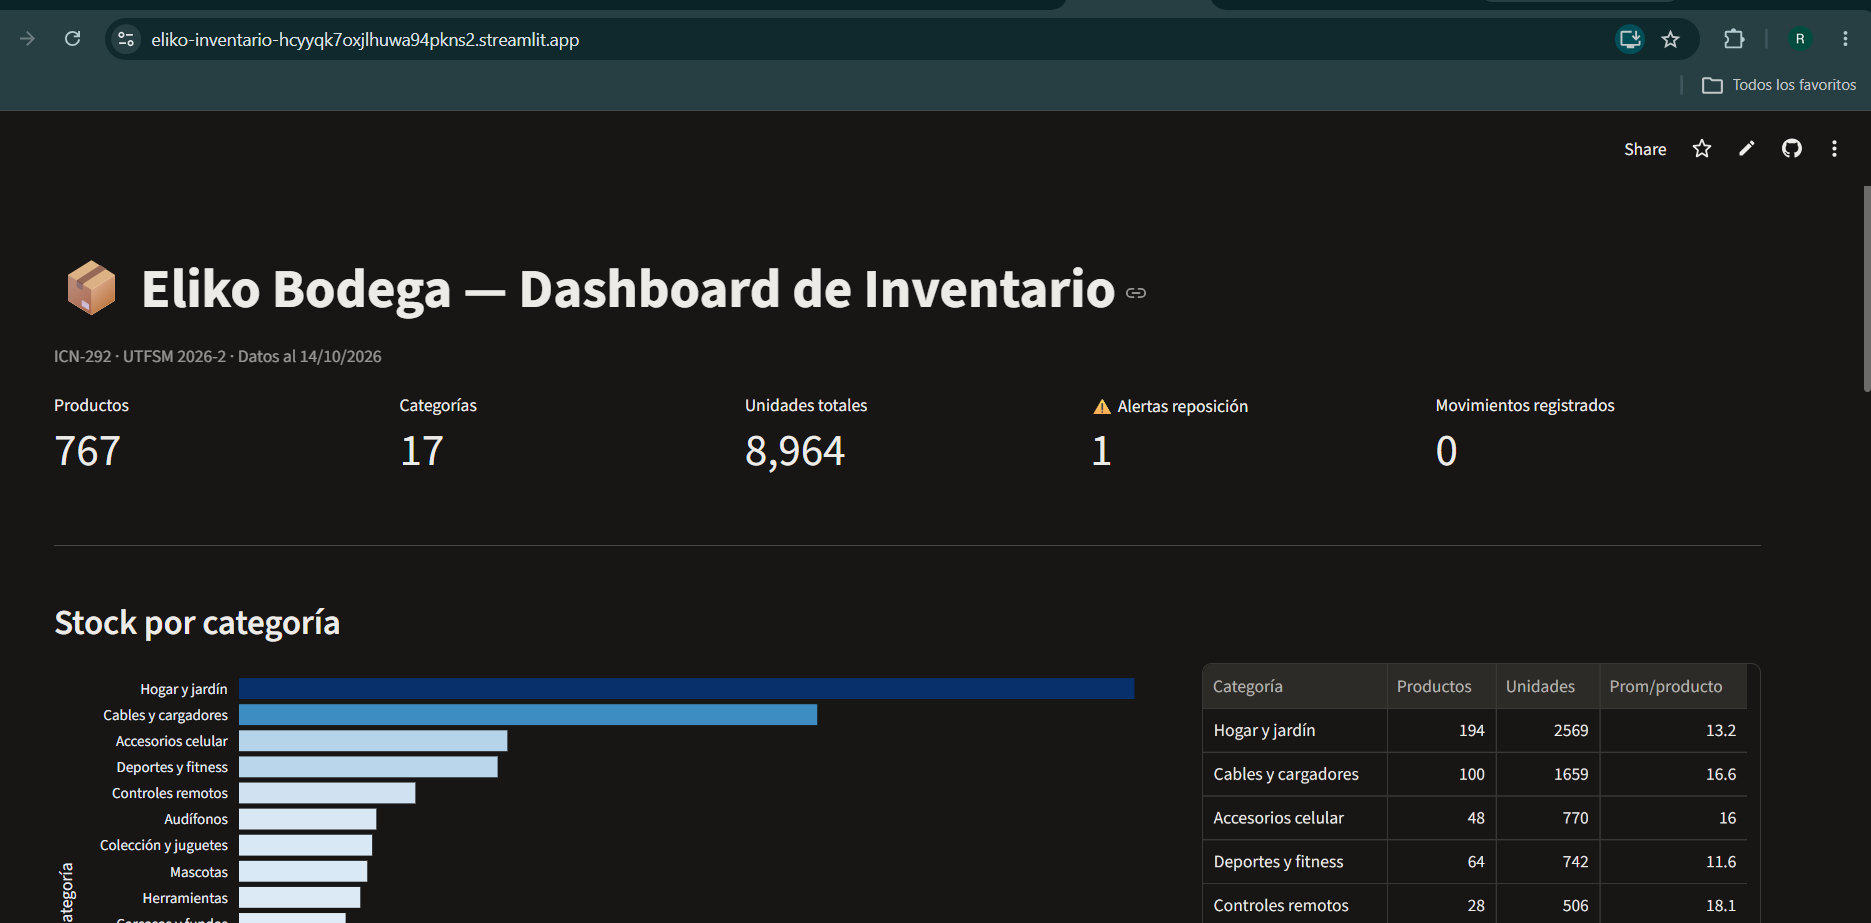
\includegraphics[width=0.95\textwidth]{img/dash1.png}
\caption{Pantalla principal del dashboard: KPIs y stock por categoría.}
\end{figure}

\section{Consultas SQL Analíticas}
La base de datos se crea con \texttt{schema.sql} (tablas, claves primarias, claves foráneas, restricciones e índices) y se carga con \texttt{seed.sql} (17 categorías, 767 productos y sus 767 registros de inventario). Las cinco consultas están en \texttt{consultas\_analiticas.sql}. Todos los resultados de esta sección se obtuvieron ejecutando:
\begin{center}
\texttt{sqlite3 -header -column eliko.db < consultas\_analiticas.sql}
\end{center}

\subsection{KPIs generales del inventario}
\begin{lstlisting}[caption={Consulta 1: KPIs generales.}]
SELECT
  (SELECT COUNT(*)          FROM producto)                      AS total_productos,
  (SELECT COUNT(*)          FROM categoria)                     AS total_categorias,
  (SELECT SUM(stock_actual) FROM inventario)                    AS total_unidades,
  (SELECT COUNT(*) FROM inventario WHERE stock_actual = 0)      AS productos_agotados,
  (SELECT COUNT(*) FROM inventario WHERE stock_minimo IS NOT NULL) AS productos_con_umbral,
  (SELECT COUNT(*)          FROM movimiento_stock)              AS total_movimientos;
\end{lstlisting}

\begin{center}
\small
\begin{minipage}{\textwidth}\centering
\captionof{table}{Resultado — Consulta 1.}
\begin{tabular}{cccccc}
\toprule
\textbf{Productos} & \textbf{Categorías} & \textbf{Unidades} & \textbf{Agotados} & \textbf{Con umbral} & \textbf{Movimientos} \\
\midrule
767 & 17 & 8.964 & 308 & 2 & 0 \\
\bottomrule
\end{tabular}
\end{minipage}
\end{center}

\textbf{Interpretación.} La bodega tiene 8.964 unidades, pero \textbf{308 de los 767 productos (40\%) están en cero}. Son publicaciones que no deberían estar activas en los canales, o que habría que reponer si se siguen vendiendo; es exactamente la situación que causa cancelaciones de venta. Además, solo 2 productos tienen un stock mínimo definido, por lo que hoy el sistema de alertas cubre una parte muy pequeña del catálogo (ver Consulta 5).

\subsection{Alertas de reposición}
\begin{lstlisting}[caption={Consulta 2: alertas de reposición.}]
SELECT p.sku, p.nombre_producto, c.nombre_categoria,
       i.stock_actual, i.stock_minimo,
       (i.stock_minimo - i.stock_actual) AS unidades_a_reponer
FROM inventario i
JOIN producto  p ON p.sku = i.sku
JOIN categoria c ON c.id_categoria = p.id_categoria
WHERE i.stock_minimo IS NOT NULL
  AND i.stock_actual < i.stock_minimo
ORDER BY unidades_a_reponer DESC;
\end{lstlisting}

\begin{center}
\small
\begin{minipage}{\textwidth}\centering
\captionof{table}{Resultado — Consulta 2.}
\begin{tabular}{llccc}
\toprule
\textbf{SKU} & \textbf{Producto} & \textbf{Stock} & \textbf{Mínimo} & \textbf{A reponer} \\
\midrule
HOG001 & Rascador Extensible Acero Inoxidable H2\ldots & 0 & 50 & 50 \\
\bottomrule
\end{tabular}
\end{minipage}
\end{center}

\textbf{Interpretación.} De los 2 productos con umbral, uno está bajo su mínimo: HOG001 está agotado y faltan 50 unidades para volver al nivel definido. El otro (CAB001) tiene 52 unidades frente a un mínimo de 12, así que no genera alerta. \texttt{WHERE stock\_minimo IS NOT NULL} evita alertas falsas en productos sin umbral, y el orden por \texttt{unidades\_a\_reponer} pone primero lo más urgente. Esta es la consulta que ejecuta el flujo n8n (§3.4).

\subsection{Stock y quiebres por categoría}
\begin{lstlisting}[caption={Consulta 3: stock y quiebres por categoría.}]
SELECT c.nombre_categoria,
       COUNT(p.sku)                                        AS productos,
       SUM(i.stock_actual)                                 AS unidades,
       ROUND(AVG(i.stock_actual), 1)                       AS promedio_unidades,
       SUM(CASE WHEN i.stock_actual = 0 THEN 1 ELSE 0 END) AS agotados,
       ROUND(100.0 * SUM(CASE WHEN i.stock_actual = 0 THEN 1 ELSE 0 END)
             / COUNT(p.sku), 1)                            AS pct_agotados
FROM categoria c
JOIN producto   p ON p.id_categoria = c.id_categoria
JOIN inventario i ON i.sku = p.sku
GROUP BY c.id_categoria, c.nombre_categoria
ORDER BY unidades DESC;
\end{lstlisting}

\begin{small}
\begin{longtable}{lrrrrr}
\caption{Resultado — Consulta 3.}\\
\toprule
\textbf{Categoría} & \textbf{Productos} & \textbf{Unidades} & \textbf{Promedio} & \textbf{Agotados} & \textbf{\% agotados} \\
\midrule
\endfirsthead
\toprule
\textbf{Categoría} & \textbf{Productos} & \textbf{Unidades} & \textbf{Promedio} & \textbf{Agotados} & \textbf{\% agotados} \\
\midrule
\endhead
\bottomrule
\endfoot
Hogar y jardín & 194 & 2.569 & 13,2 & 132 & 68,0 \\
Cables y cargadores & 100 & 1.659 & 16,6 & 44 & 44,0 \\
Accesorios celular & 48 & 770 & 16,0 & 4 & 8,3 \\
Deportes y fitness & 64 & 742 & 11,6 & 18 & 28,1 \\
Controles remotos & 28 & 506 & 18,1 & 15 & 53,6 \\
Audífonos & 34 & 394 & 11,6 & 0 & 0,0 \\
Colección y juguetes & 29 & 382 & 13,2 & 5 & 17,2 \\
Mascotas & 38 & 368 & 9,7 & 5 & 13,2 \\
Herramientas & 25 & 348 & 13,9 & 13 & 52,0 \\
Carcasas y fundas & 95 & 306 & 3,2 & 28 & 29,5 \\
Memorias y almacen. & 51 & 266 & 5,2 & 35 & 68,6 \\
Belleza & 15 & 186 & 12,4 & 0 & 0,0 \\
Relojes & 22 & 151 & 6,9 & 3 & 13,6 \\
Equipos satelitales & 10 & 111 & 11,1 & 2 & 20,0 \\
Salud & 4 & 109 & 27,3 & 0 & 0,0 \\
Computación & 8 & 97 & 12,1 & 2 & 25,0 \\
Intercomunicadores & 2 & 0 & 0,0 & 2 & 100,0 \\
\end{longtable}
\end{small}

\textbf{Interpretación.} “Hogar y jardín” es la categoría más grande (194 productos y 2.569 unidades), pero también la que tiene más quiebres: 132 productos agotados (68\%). Lo mismo ocurre con “Memorias y almacenamiento” (68,6\%) y “Controles remotos” (53,6\%). En cambio, “Audífonos”, “Belleza” y “Salud” no tienen productos agotados. Para Alejandro, esto indica dónde revisar primero las publicaciones activas y dónde concentrar las compras: el problema no es la falta de unidades en general, sino que están concentradas en pocos productos.

\subsection{Productos con mayor stock}
\begin{lstlisting}[caption={Consulta 4: top 10 productos con mayor stock.}]
SELECT p.sku, p.nombre_producto, c.nombre_categoria, i.stock_actual
FROM inventario i
JOIN producto  p ON p.sku = i.sku
JOIN categoria c ON c.id_categoria = p.id_categoria
ORDER BY i.stock_actual DESC
LIMIT 10;
\end{lstlisting}

\begin{center}
\small
\begin{minipage}{\textwidth}\centering
\captionof{table}{Resultado — Consulta 4.}
\begin{tabularx}{\textwidth}{l X l r}
\toprule
\textbf{SKU} & \textbf{Producto} & \textbf{Categoría} & \textbf{Stock} \\
\midrule
HOG015 & 2 Soportes pequeños GYM de acero galvanizado (kit doble) & Hogar y jardín & 296 \\
HOG010 & 2 Soportes para hamaca de acero galvanizado (kit grande) & Hogar y jardín & 278 \\
CAB053 & Grampas RG6 blancas 100 unid. para cable coaxial & Cables y cargadores & 197 \\
CAB016 & Kit 100 bridas precintos clip automotriz & Cables y cargadores & 196 \\
HOG066 & Resorte acero inoxidable para hamacas y columpios & Hogar y jardín & 192 \\
ACC003 & Soporte clip para intercomunicador Ejeas V6pro & Accesorios celular & 186 \\
HOG132 & Bolsa para aspiradora universal de tela & Hogar y jardín & 159 \\
HOG011 & Kit de soporte para silla colgante y hamacas & Hogar y jardín & 148 \\
HOG025B & Enchufe corriente americano a nacional 220v & Hogar y jardín & 137 \\
CTR007G & Control remoto genérico para Android & Controles remotos & 129 \\
\bottomrule
\end{tabularx}
\end{minipage}
\end{center}

\textbf{Interpretación.} Estos 10 productos suman 1.918 unidades, es decir, \textbf{el 21\% del stock total está en el 1,3\% de los productos}. Seis de ellos son de “Hogar y jardín”, la misma categoría con más agotados: dentro de una categoría conviven productos con exceso y productos en cero. Es información útil para no volver a comprar lo que sobra y priorizar lo que falta.

\subsection{Productos en stock crítico sin umbral configurado}
\begin{lstlisting}[caption={Consulta 5: stock crítico sin umbral, por categoría.}]
SELECT c.nombre_categoria,
       COUNT(*)                                            AS productos_criticos_sin_umbral,
       SUM(CASE WHEN i.stock_actual = 1 THEN 1 ELSE 0 END) AS con_1_unidad,
       SUM(CASE WHEN i.stock_actual = 2 THEN 1 ELSE 0 END) AS con_2_unidades
FROM inventario i
JOIN producto  p ON p.sku = i.sku
JOIN categoria c ON c.id_categoria = p.id_categoria
WHERE i.stock_minimo IS NULL
  AND i.stock_actual BETWEEN 1 AND 2
GROUP BY c.id_categoria, c.nombre_categoria
ORDER BY productos_criticos_sin_umbral DESC;
\end{lstlisting}

\begin{center}
\small
\begin{minipage}{\textwidth}\centering
\captionof{table}{Resultado — Consulta 5.}
\begin{tabular}{lrrr}
\toprule
\textbf{Categoría} & \textbf{Críticos sin umbral} & \textbf{Con 1 unidad} & \textbf{Con 2 unidades} \\
\midrule
Carcasas y fundas & 25 & 11 & 14 \\
Accesorios celular & 9 & 3 & 6 \\
Mascotas & 7 & 4 & 3 \\
Hogar y jardín & 6 & 2 & 4 \\
Audífonos & 5 & 3 & 2 \\
Deportes y fitness & 5 & 1 & 4 \\
Colección y juguetes & 4 & 2 & 2 \\
Equipos satelitales & 3 & 3 & 0 \\
Belleza, Cables y cargadores, Relojes & 2 c/u & 1 c/u & 1 c/u \\
Computación & 1 & 1 & 0 \\
Memorias y almacen. & 1 & 0 & 1 \\
\midrule
\textbf{Total} & \textbf{72} & \textbf{33} & \textbf{39} \\
\bottomrule
\end{tabular}
\end{minipage}
\end{center}

\textbf{Interpretación.} Hay \textbf{72 productos con solo 1 o 2 unidades que el sistema no puede alertar}, porque no tienen stock mínimo definido. Son los quiebres más probables de las próximas semanas, en especial en “Carcasas y fundas” (25 productos). La acción concreta para Eliko es definir primero el umbral de estos 72 productos: así el flujo n8n empieza a avisar justo donde hoy existe más riesgo de cancelar una venta.

\section{Repositorio GitHub y guía de uso}
\textbf{URL:} \url{https://github.com/benjaminmaturanab-create/ICN292-GRUPO4-Barros-Fuentes-Lopez-Uribe-Maturana}

Este es el repositorio único del proyecto: contiene los entregables de la E1 y de la E2, y es el que se audita en la defensa.

El paso a paso completo está en el \texttt{README.md} del repositorio. En resumen, en un computador con Python 3 y Git:
\begin{enumerate}[leftmargin=1.6em]
\item \textbf{Clonar el repositorio:}\\ \texttt{git clone} \path{https://github.com/benjaminmaturanab-create/ICN292-GRUPO4-Barros-Fuentes-Lopez-Uribe-Maturana}
\item \textbf{Instalar dependencias:} \texttt{pip install -r requirements.txt}
\item \textbf{Crear y cargar la base:} \texttt{sqlite3 eliko.db < schema.sql} y luego \texttt{sqlite3 eliko.db < seed.sql}. Si el computador no tiene el programa \texttt{sqlite3}, el \texttt{README.md} incluye una alternativa de una línea en Python.
\item \textbf{Ejecutar las consultas de negocio:} \texttt{sqlite3 -header -column eliko.db < consultas\_analiticas.sql}
\item \textbf{Abrir el dashboard:} \texttt{streamlit run app.py}
\item \textbf{Automatización:} en n8n Cloud, importar \path{n8n/flujo_alerta_stock_cloud.json}, conectar la cuenta de Gmail en el nodo de correo y ejecutar el flujo (detalle en \path{docs/05-automatizacion-n8n.md}).
\end{enumerate}

\section{Reflexión Ética}
\subsection{Uso de inteligencia artificial}
Se usó IA generativa (Claude, de Anthropic) como apoyo para escribir el esquema SQL a partir del ER diseñado por el equipo, convertir el CSV del inventario a sentencias \texttt{INSERT}, escribir y depurar el código del dashboard, diseñar el flujo n8n y redactar este informe. \textbf{La IA no inventó datos:} todos los valores de \texttt{seed.sql} provienen del inventario levantado por el equipo, con las reglas de limpieza de la §8.2. El equipo ejecutó y verificó todo lo entregado, y el detalle está en \texttt{DECLARACION\_IA.md}.

\subsection{Origen y tratamiento de los datos}
Los datos provienen del \textbf{inventario físico que el equipo realizó en la bodega de Eliko} (octubre–noviembre 2026), con autorización de la empresa para fines académicos. El archivo \texttt{Inventario\_Bodega\_Eliko\_14\_10\_2026.csv} (768 filas) se cargó con estas reglas, también documentadas en el \texttt{README.md}: 1 fila sin SKU se omitió; 73 productos sin nombre se cargaron como “Producto \{SKU\}”; 23 productos sin categoría la recibieron según el prefijo de su SKU; y 2 notas de texto en el stock mínimo (“revisar 24 piezas”) quedaron sin umbral. Los datos se usan solo para el fin académico declarado.

\section{Lecciones Aprendidas y Limitaciones}
\subsection{Lecciones aprendidas}
\begin{itemize}
\item \textbf{Primero datos confiables, después automatización.} Descontar stock por canal no sirve si el stock de partida es incorrecto; el conteo en terreno fue el paso que habilitó todo lo demás y debió hacerse antes.
\item \textbf{Ajustar el alcance al tiempo disponible.} La E1 proponía 10 entidades y un stack de cuatro capas; 4 tablas bien normalizadas y un stack simple permitieron entregar un sistema que funciona.
\item \textbf{Las alertas dependen de sus parámetros.} La lógica funciona, pero con umbral definido en solo 2 productos el sistema casi no puede avisar. Definir los mínimos con el dueño es tan importante como programar la alerta.
\item \textbf{Medir el impacto económico para priorizar.} Alejandro veía como mayor carga crear publicaciones, pero las pérdidas por cancelaciones mostraron que el quiebre de stock era más crítico.
\item \textbf{Documentar a partir de lo que corre.} El modelo cambió durante el desarrollo (se agregó la tabla INVENTARIO), y hubo que alinear el ER, las consultas y el informe con la base real. Todo resultado debe salir de ejecutar el código.
\end{itemize}

\subsection{Limitaciones}
\begin{small}
\begin{longtable}{>{\raggedright\arraybackslash}p{4.2cm} >{\raggedright\arraybackslash}p{10.9cm}}
\toprule
\textbf{Limitación} & \textbf{Consecuencia} \\
\midrule
\endfirsthead
\toprule
\textbf{Limitación} & \textbf{Consecuencia} \\
\midrule
\endhead
\bottomrule
\endfoot
Sin integración con los canales & La venta simultánea de la última unidad en dos plataformas todavía no se evita: el stock de cada canal se actualiza a mano. \\
Sin formulario de movimientos & Entradas y salidas se registran por SQL (hoy hay 0), por lo que el descuento automático (RF02) no opera y aún no se puede medir si bajaron las cancelaciones. \\
Umbrales en 2 de 767 productos & Solo esos 2 productos pueden generar alerta; 72 con 1–2 unidades quedan fuera (§6.5). \\
Base no persistente en la nube & Streamlit Cloud regenera la base al reiniciar, así que un movimiento registrado en línea se perdería. \\
Sin autenticación & Cualquiera con el enlace ve el dashboard; es requisito antes de guardar datos personales (Ley 21.719). \\
\end{longtable}
\end{small}

\end{document}
